\section{Introduction}
\label{sec:intro}


\iffalse
\begin{figure}[t]
\centering
	\subfloat[Unordered communication.\label{fig:lightcone-traditional}]
	{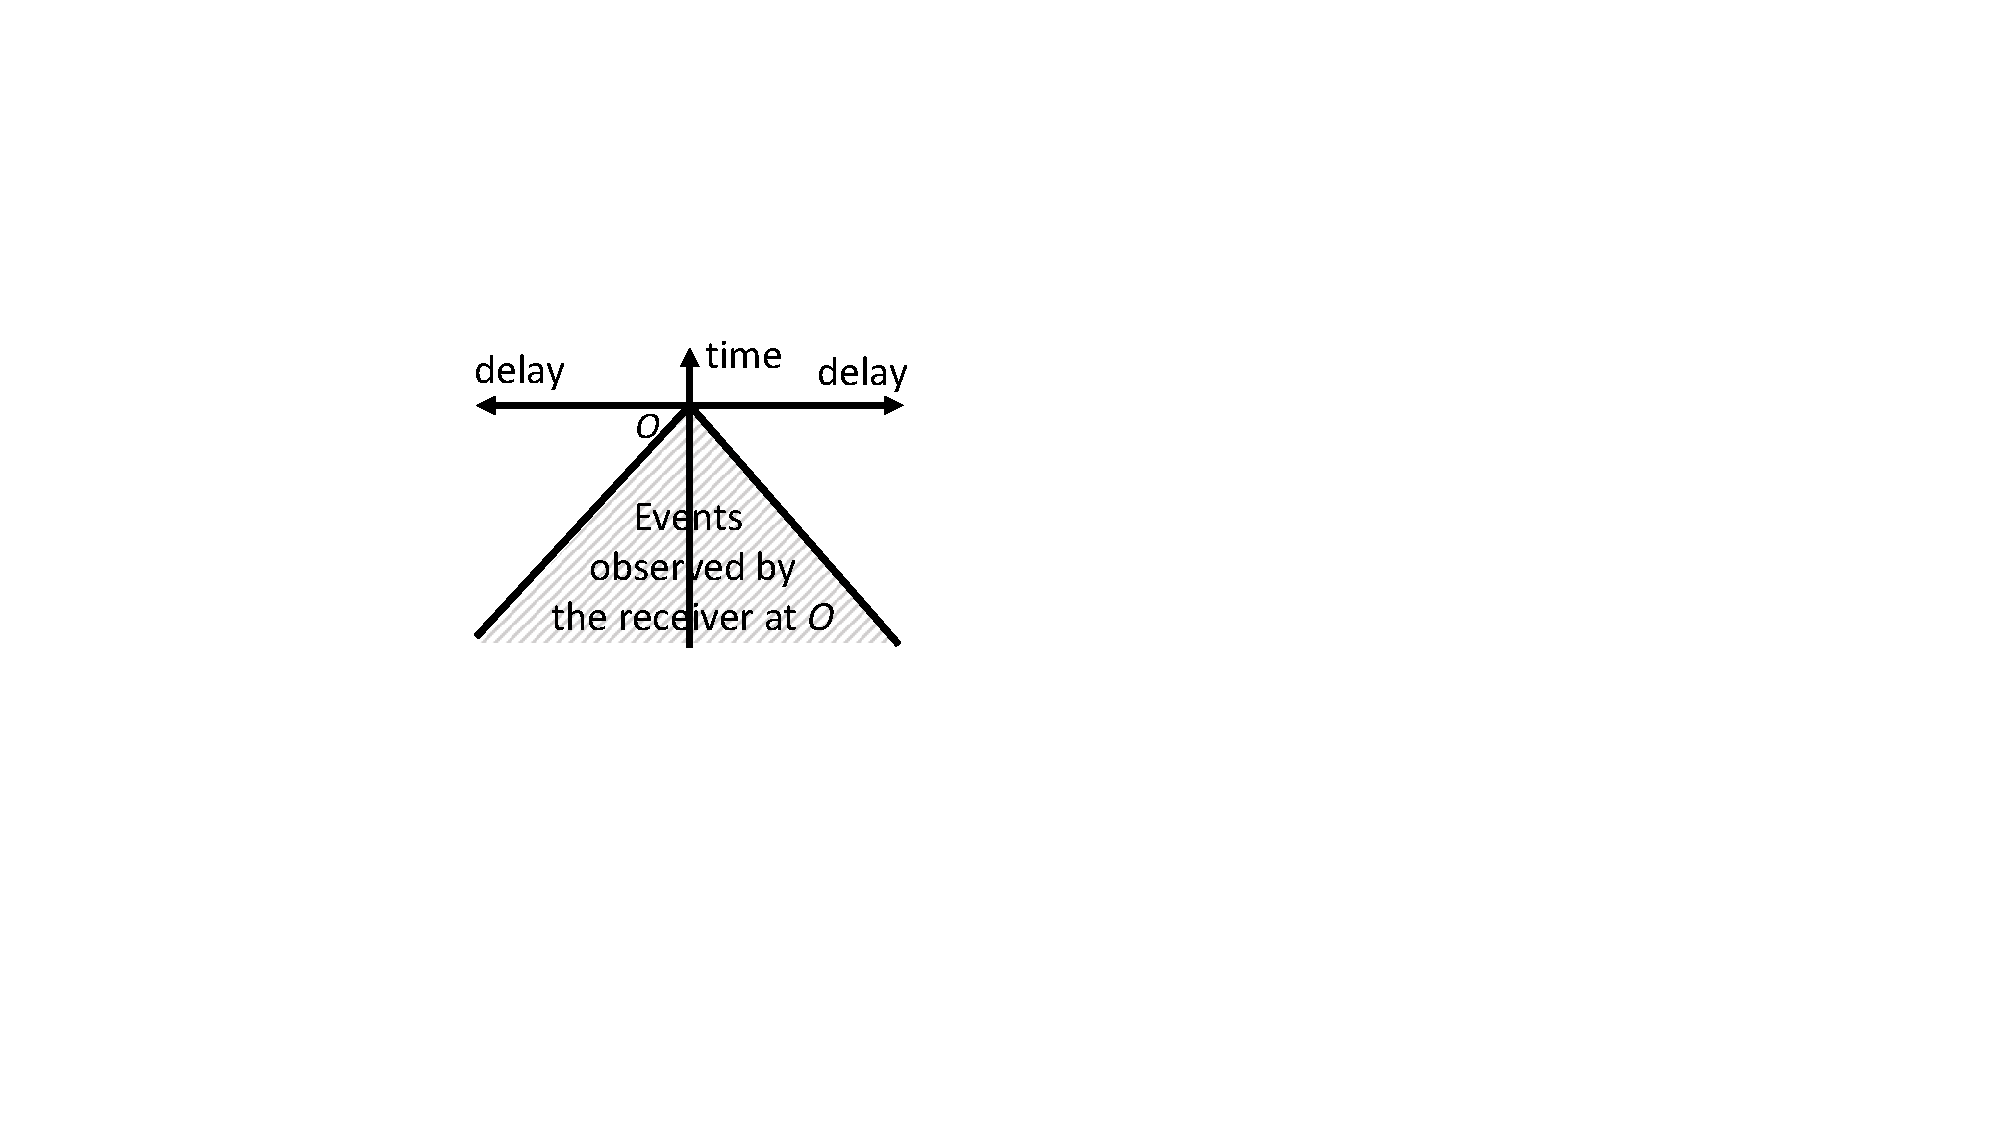
\includegraphics[width=.23\textwidth,page=1]{images/cropped_lightcone.pdf}}
	\subfloat[Total order communication.\label{fig:lightcone-toms}]
	{\includegraphics[width=.23\textwidth,page=2]{images/cropped_lightcone.pdf}}
	\caption{Light cone of observed events by a receiver.}
	\label{fig:lightcone}
    \vspace{-15pt}
\end{figure}
\fi

The lack of total order communication often complicates distributed system design.
For example, when a host atomically reads or writes multiple objects on different remote hosts, there is no guarantee that the messages arrive at different remote hosts at the same time, so, locks are often required to achieve consistency.
As another example, multiple shards of a distributed database generate logs to multiple replicas, and each replica may receive logs from the shards in a different interleaving ordering, thus violating data consistency.
%A centralized sequencer can solve this problem, but it introduces a central bottleneck.

%Today's data centers host a variety of distributed systems~\textcolor{red}{cite some papers here} to provide service for global users. 
%In a network with arbitrary delays, messages are not guaranteed to be delivered in a consistent order.
%For example, multiple shards of a distributed database generate logs to multiple replicas.
%Each replica may receive logs from shards in a different order.
%Without special care, such inconsistent ordering may violate data consistency.
%Solutions that mitigate this problem often introduce synchronization overhead, and often complicate distributed system design.

%\textcolor{red}{describe side effects, e.g., violating data consistence}.
%For example, multiple shards of a distributed database generate logs to multiple replicas, and each replica may receive logs from the shards in a different interleaving ordering.
%The ability to order events in a distributed system is essential for the correctness of many distributed protocols~\cite{lamport1978time,chandy1985distributed}.

%Total order communication provides an abstraction where different receivers process messages from senders in a consistent order. In a total order communication system, messages are tagged with monotonic \textit{event timestamps} by sender, and each receiver processes all messages sent to it based on timestamp order. In log replication, each replica will receive logs in a consistent ordering, which can be an important building block for both strongly consistent and eventually consistent systems. In addition, total order communication can improve consistency in distributed shared memory, as well as accelerate transactional key-value stores~\cite{ports2015designing, eris}, fault-tolerant consensus~\cite{li2016just} and state machine replication~\cite{state-machine-replication}.



In this work, we propose \sys{}, a communication primitive that provides ``one big pipe'' abstraction in a data center network (DCN). As Figure~\ref{fig:1pipe} shows, messages are sent in batches and serialized in a virtual pipe, which enables different receivers to process messages from senders in a consistent order.
More precisely, \sys{} resembles Causally and Totally Ordered Communication Support (CATOCS)~\cite{cheriton1994understanding}: (1) messages are \emph{totally ordered}, ensuring that they are delivered in the same order to all receivers; (2) messages are delivered obeying the \emph{causal order} in the Lamport logic clock sense~\cite{lamport1978time}. In addition to unicast, \sys{} also supports \emph{scattering}, which groups multiple messages to different receivers at the same position of the total order. Different from traditional multicast, each message in a scattering has distinct content and destination. Users do not need to define multicast channels or groups because the network is a big CATOCS channel.


\begin{figure}[t]
	\centering
	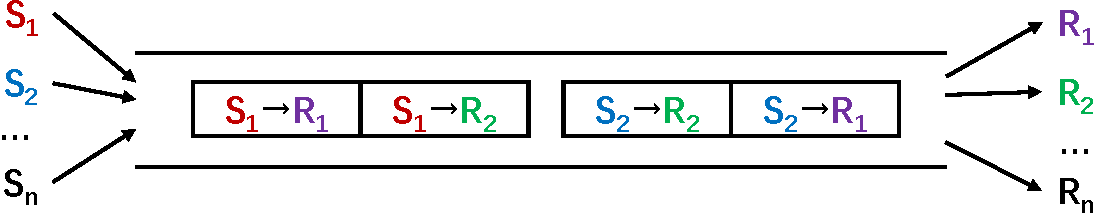
\includegraphics[width=.45\textwidth]{images/1pipe.pdf}
	\caption{\sys{} abstraction.}
	\label{fig:1pipe}
\end{figure}


\sys{} can achieve distributed atomic multi-object read and write with a single scattering because they are delivered at the same logical time. Replication in \sys{} takes one round-trip time (RTT). \sys{} also provides a total ordering of communication events, thus reducing fences and improving concurrency of distributed systems.


%Besides ordering, another desirable abstraction is a reliable communication system that is able to deliver a group of messages atomically: either all the messages in a group are delivered to the desired targets, or non is delivered. 
%Since the dawn of distributed system research~\cite{lamport1978time}, many efforts have been made to achieve atomic broadcast and multicast~\cite{defago2004total}. However, existing solutions suffer from scalability or efficiency limitations~\cite{eris,rajagopalan1989token,kim1997total,ekwall2004token,lamport1978time,birman1985replication,chandra1996unreliable}. 
%One line of work leverages logically centralized coordination, \textit{e.g.}, centralized sequencers~\cite{eris}, or tokens to be passed among senders and receivers~\cite{rajagopalan1989token,kim1997total,ekwall2004token}. As a result, it is challenging to scale the system. Another line of work uses fully distributed coordination, \textit{e.g.}, exchange timestamps among receivers before they start to process messages~\cite{lamport1978time,birman1985replication,chandra1996unreliable}. This causes extra network communication overhead and delay, thus degrading system efficiency. Moreover, an additional restriction comes from the semantics of multicast, where all the receivers must receive identical messages.

%In this work, we propose Reliable Ordered Message Scattering (\sys), an efficient and scalable method to scatter groups of messages reliably. We generalize multicast to \emph{message scattering}~\cite{kshemkalyani2011distributed}, a communication pattern where a host sends a group of (potentially different) messages to multiple hosts simultaneously. \sys strictly preserves the following two properties in an efficient and scalable manner:
%\begin{ecompact}
%\item \textbf{Ordering}: Each receiver delivers messages from different senders in the ascending wall clock order of message sent time.
%Wall clock is a clock on each host that obeys monotonicity and causality, that is (not strictly) synchronized.
%This implies CATOCS.
%\item \textbf{Reliability}: It means both (1) \emph{atomicity}, i.e., either all or none receivers deliver messages in a scattering group, and (2) \emph{validity}, i.e., a scattering is guaranteed to be delivered if all the senders and receivers are not faulty, and the network is not partitioned.
%\end{ecompact}

%The \sys primitive can support externally consistent distributed transactions~\cite{ports2015designing, eris}, replication in eventually consistent systems, state machine replication~\cite{state-machine-replication} as well as improve consistency in distributed shared memory. 

%Total order communication provides an abstraction where different receivers process messages from senders in a consistent order~\cite{kshemkalyani2011distributed}.
%More formally, in total order communication, for each pair of hosts $R_i$ and $R_j$ and for each pair of messages $M_x$ and $M_y$ that are delivered to both hosts, $R_i$ is delivered $M_x$ before $M_y$ if and only if $R_j$ is delivered $M_x$ before $M_y$.
%Ordered communication provides an abstraction where different receivers process messages from senders in a consistent order. This abstraction, sometimes called Causally and Totally Ordered Communication Support (CATOCS)~\cite{cheriton1994understanding}, 
%In a total order communication system, messages are tagged with monotonic \textit{event timestamps} by the sender. The receiver processes arrival messages based on the timestamp order. In log replication, each replica will process logs in a consistent order, which can be 
%is an important building block for both strongly consistent and eventually consistent systems. Ordered communication provides the guarantee that messages are delivered obeying the \emph{causal order} in the Lamport logic clock sense~\cite{lamport1978time}. This also imply \emph{FIFO}, i.e., if a message is sent after the other, it will also be delivered before the other. Moreover, messages are \emph{total order}, ensuing that they are delivered in the same order to all participants. 
%The primitive can improve consistency in distributed shared memory, as well as accelerate transactional key-value stores~\cite{ports2015designing, eris}, fault-tolerant consensus~\cite{li2016just} and state machine replication~\cite{state-machine-replication}.


%Totally ordered message scattering provides an abstraction with a new view of space-time, where different receivers process messages scattered from senders in a consistent order (Figure~\ref{fig:light-cone} (b)). In a total order message scattering system, messages are total order with \textit{event timestamps}, and each receiver receives all messages scattered to it in the timestamp order. This can simplify and accelerate many distributed applications, \textit{e.g.}, transactional key-value stores~\cite{ports2015designing, eris}, total store ordering in distributed shared memory~\cite{}, fault-tolerant consensus~\cite{li2016just}, mutual exclusion~\cite{lamport1978time}, state machine replication~\cite{lamport1978time,lamport1978implementation} and distributed snapshots~\cite{chandy1985distributed}.

%The ordering of events is fundamental to distributed systems.
%The ability to \textit{total order} events in a distributed system, \textit{i.e.}, all nodes observe a consistent ordering of all events, can lead to simple and efficient implementation of a wide range of distributed applications, \textit{e.g.}, transaction processing~\cite{ports2015designing, eris}, transactional key-value stores~\cite{ports2015designing, eris}, fault-tolerant consensus~\cite{li2016just}, mutual exclusion~\cite{lamport1978time}, state machine replication~\cite{lamport1978time,lamport1978implementation} and distributed snapshots~\cite{chandy1985distributed}.
%A total ordering of events indicates that each event can be tagged with a \RED{\textit{logical timestamp}}, and each node observes events in increasing timestamp order (break ties by origin node ID).

%In a networked system, effects of an event propagate via network messages. This means to \textit{scatter} messages from the origin node to a set of receiver nodes. For communication efficiency, an event may not need to be observed by all nodes, and different nodes may receive different messages originated from a same event, so generally it is a \textit{scattering} instead of a \textit{broadcast} or \textit{multicast}. Messages are tagged with the timestamp of the origin event. A node observes an event by receiving the corresponding message. Consequently, from a receiver's perspective, \textit{total ordering of input message timestamps implies total ordering of its observed events}.

%Many efforts have been made to achieve reliable and ordered group communication, namely atomic broadcast and multicast~\cite{defago2004total}.
%Most existing works are designed for a small-to-medium group of known and trusted hosts, where each client sends the same message to every participant.
%However, distributed systems in data centers scale to thousands of hosts~\cite{nishtala2013scaling}, while each client communicate with a small and non-predetermined subset of hosts for each scattering.
%To this end, we design \sys for a very large group of unknown and untrusted hosts in data centers.
%In this scenario, existing solutions suffer from scalability, efficiency or security limitations.


%Since the dawn of distributed system research~\cite{lamport1978time}, many efforts have been made to achieve ordered broadcast and multicast~\cite{defago2004total}.
%In this paper, we consider a more general form of communication, namely \emph{message scattering}. Message scattering is a common communication pattern where a sender sends (potentially different) messages to multiple receivers. In contrast, identical messages are sent in multicast and broadcast. In a total order message scattering system, different receivers will process scattered messages in a consistent order. Assume $S_1$ scatters $M_1, M'_1$ and $S_2$ scatters $M_2, M'_2$. If $M_1$ is processed before $M_2$ at receiver $A$, then the same processing order should be kept at receiver $B$, \textit{i.e.}, $B$ will process $M'_1$ before $M'_2$.
%Most total order multicast algorithms can be used to implement total order message scattering with some modifications.
%However, existing solutions suffer from scalability or efficiency limitations.
%One line of work leverages logically centralized coordination, \textit{e.g.}, centralized sequencers~\cite{eris}, or tokens to be passed among senders and receivers~\cite{rajagopalan1989token,kim1997total,ekwall2004token}.
%As a result, it is challenging to scale the system.
%Another line of work uses fully distributed coordination, \textit{e.g.}, exchange timestamps among receivers before they start to process messages~\cite{lamport1978time,birman1985replication,chandra1996unreliable}.
%This causes extra network communication overhead and delay, thus degrading system efficiency.
%An additional limitation comes from the semantics of multicast, where each receiver must get a same sequence of messages. 
%Moreover, an additional restriction comes from the semantics of multicast, where all the receivers must receive identical messages.

%In this work, we seek a solution to provide scalable and efficient reliable ordered communication for distributed systems in a data center environment, where the network is regular and switches have generally good programmability .
%Message scattering is common in distributed systems.
%For instance, in distributed storage, a client writes metadata to a site and data to another site, while another client reads them concurrently. Consistency between metadata and data requires the operations to be scattered atomically to the two sites.

%For instance, web servers send an access log and an error log of each HTTP request to different log collectors. Achieving consistent ordering of requests between access and error logs requires \textit{total-order message scattering} (\sys), which ensures a group of messages to be scattered atomically.
%Assume $S_1$ scatters access log $A_1$ and error log $E_1$, while $S_2$ scatters $A_2$ and $E_2$. If $A_1$ is processed before $A_2$ at access log collector, then error log collector should process $E_1$ before $E_2$.
%Logically, a \sys network resembles a FIFO where messages in a same \textit{scattering} are enqueued atomically, and messages are dequeued by receivers in FIFO order.

%Since the dawn of distributed systems research~\cite{lamport1978time}, there has been considerable amount of literature on total-ordering events and input messages using \textit{total order broadcast}~\cite{defago2004total}.
%Most total-order broadcast algorithms can be modified to implement total-order message scattering, but they have scalability or efficiency limitations.
%One line of work uses logically centralized coordination, \textit{e.g.}, using one or more centralized sequencers~\cite{eris}, or have a token to be passed among senders or receivers~\cite{}. The throughput of such systems is hard to scale.
%Another line of work uses fully distributed coordination, \textit{e.g.}, add a consensus round among receivers after they receive the messages~\cite{}. The network communication overhead and additional consensus delay are not negligible.

%Data center network (DCN) has many desirable properties for distributed systems design, such as regular topologies~\cite{leiserson1985fat,greenberg2009vl2} and single administrative domain.
%Furthermore, programmable switches start to flourish in data centers, providing more flexible packet processing.
%Recently, there has been a trend to co-design distributed systems with underlying data center networks~\cite{eris,netcache-sosp17,dang2016paxos}.
%\sys follow this trend and take advantage of a programmable data center network.

%In \sys, hosts send messages to other hosts. A timestamp is attached to every message by the sender. The timestamps satisfy two requirements. First, for a given host the timestamps are non-decreasing, meaning that when a host sends out two messages, the latter one will have a timestamp equal or larger than that of the first one. Messages sent by a host with the same timestamp are considered to form a scattering group. Second, the timestamps satisfy causality property, meaning that when \sys delivers a message to a host, it guarantees that all future messages sent by the host will have timestamps larger than that of the delivered message. \sys achieves reliable ordered message delivery. Unless the host is faulty or unreachable, all messages sent to a particular host will be delivered exactly once according to the timestamp order.  

\sys{} seems to require a central serialization point, which is not scalable.
In this work, we propose a scalable and efficient implementation of \sys{} in a DCN, where the topology is regular~\cite{leiserson1985fat,greenberg2009vl2}, and switches have generally good programmability.
Our principle is to co-design end hosts with the underlying DCN.
We synchronize the clocks on hosts and ensure they are non-decreasing.
The sender attaches a same timestamp to each packet in a unicast message or scattering.
%The timestamps satisfy two reqirements.
%First, for a given host the timestamps are non-decreasing.
%Messages sent by a host with the same timestamp are considered to form a scattering.
%Second, the timestamps satisfy causality property, meaning that when \sys delivers a message to a host, it guarantees that all future messages sent by the host will have timestamps larger than that of the delivered message.
Each receiver delivers messages in non-decreasing timestamp order.


At its core, \sys separates the bookkeeping of order information from message forwarding.
\sys forwards timestamped packets as usual in the network, and buffers them at the receiver side.
The key challenge is to let a receiver know that all packets below a certain timestamp has arrived.
To this end, we introduce a \emph{barrier} timestamp on each link and switch, which is essentially the \emph{lower bound} of the timestamps of all future arrival packets.
Each switch aggregates barrier information of all ingress links to derive the barrier for all egress links.
In this way, barriers propagate in the DAG network, and the receiver can deliver the messages with timestamps below the barrier in order.
If some hosts or links are temporarily idle, we periodically generate \emph{beacons} carrying barrier information.

Regarding packet loss and failures, \sys{} provides a \emph{best effort} service in which each message is delivered at most once; and a \emph{reliable} service in which a message is guaranteed to be delivered if both sender and all receivers in the scattering are correct.
In addition, reliable \sys{} ensures \emph{restricted failure atomicity}: either all or none messages in a scattering are delivered unless a receiver fails permanently or network partitions after the messages are sent.
Reliable \sys{} uses a two-phase commit (2PC) approach, where the first phase is end-to-end packet loss recovery, and the second phase aggregates \emph{commit barriers} through the network.
It relies on a highly available network controller to coordinate failure handling.
Reliable \sys{} adds one round-trip time (RTT) compared to best effort \sys{}.

\iffalse
To take advantage of the fact that data centers are typically well engineered and have very low packet loss rates~\cite{ports2015designing}, when packet loss does not occur, a host can \emph{reliably deliver} a message when it is sure that all hosts have received messages with lower timestamps.
To this end, a receiver responds an ACK for each message, and the switch aggregate \emph{ACK barriers} from receivers to senders (Sec.\ref{sec:ack-barrier}).
When packet loss is detected, hosts stop delivering messages according to loss-free and ACK barriers.
After retransmission, we aggregate \emph{delivery barriers} from senders to receivers to resume reliable delivery and reset loss detectors (Sec.\ref{sec:lossy}).

To achieve consensus under failures of hosts, rather than voting, we use the top-of-rack switch of each host to reliably detect host failures via beacon timeout.
Host failure information is reliably propagated through the network along with delivery barriers (Sec.\ref{sec:host-failure}).
After failure recovery, a host can rejoin the system (Sec.\ref{sec:failure-recovery}).
To ensure security, the top-of-rack switches enforce the hosts comply with \sys protocol, so Byzantine failures of hosts can also be detected (Sec.\ref{sec:byzantine}).
Crash failures of network switches and links would stall the system but not violate correctness.
To ensure liveness, we rely on the centralized SDN controller to resume operation of a largest strongly connected network partition (Sec.\ref{sec:network-failure}).
\fi


%At its core, \sys separates the bookkeeping of order information from message forwarding.
%\sys attaches a timestamp to each message at the sender side, forwards them as usual in the network, and buffers them at the receiver side.
%The switch aggregates timestamp information of all messages to derive the \textit{barrier} for each receiver.
%The barrier is essentially the \textit{lower bound} of the timestamps of all future arrival packets.
%With this information, the receiver can deliver the messages with timestamps below the barrier in order.
%\sys is scalable as the switches and end hosts form a decentralized system where control plane communication only takes place between directly connected nodes.

%To ensure \sys's efficiency and reliability, we still need to solve three main challenges: 1) How to derive timestamp barriers? 2) How to assign event timestamps? and 3) How to handle packet losses and node failures?

%For the first challenge, we first generalize timestamp barriers from end hosts to every link in the network.
%Each switch keeps per-link barrier information and updates it for each packet.
%We merge barriers hierarchically at switches to reduce communication overhead (Sec.\ref{sec:ideal}).
%If some hosts or links are temporarily idle, we periodically generate beacons carrying barrier information (Sec.\ref{sec:beacon}).


%To reduce delay, messages from different senders should be delivered to a host at about the same time if and only if they are sent at around the same wall clock time.
%Therefore, an obvious candidate for event timestamp would be (potentially synchronized) local physical clock of each host.
%However, this does not account for the network latency difference incurred by the OS and links, thus makes fast links constantly waiting for slow links.
%%For example, two messages are transmitted from two senders to the same receiver at the same physical time. However, they arrive at different times due to their different network path lengths. As a result, the earlier one must wait for the later one to be processed together.
%To minimize the impact, we propose \textit{minimax clock synchronization} (Sec.\ref{sec:sync}) to synchronize logical clocks on each node and assign timestamps to events according to the logical clocks.

%For the third challenge, we take advantage of the fact that data centers are typically well engineered and have very low packet loss rates~\cite{ports2015designing}.
%We detect packet loss via counters in network switches, and rely on end hosts to retransmit lost packets (Sec.\ref{sec:lossy}).
%We detect failures of hosts, switches and links via beacon timeout.
%When no packet loss or failure is present, a message scattering can be delivered in just one network delay. Otherwise, we fall back to two-phase commit (2PC) to deliver a scattering in three network delays (Sec.\ref{sec:failure}).

%In Sec.\ref{sec:lossy}, we add reliability to total-order message scattering in lossy networks, with overhead of one round-trip delay. 


%A simple existing approach to total order messages to the end hosts is called \textit{determin istic merge}~\cite{hadzilacos1994modular, aguilera2000efficient}, which serialize network messages at each network switch. However, commodity switches do not have enough buffer capacity and the programmability to \textit{merge sort} ingress streams (cite PIFO).

%In this work, we propose a different approach to achieve total order scattering. The messages are forwarded as normal in network switches and buffered in end-host receivers. Network switches aggregate timestamp \textit{barrier} information to indicate the \textit{lower bound} of all future timestamps that can be received by an end host. The end hosts reorder messages below the timestamp barrier and deliver them to applications.
%Two challenges arise: \textit{How to derive timestamp barriers? How to assign event timestamps?}

%To derive timestamp barriers, we generalize timestamp barriers from end hosts to every link in the network. A barrier packet on a link indicates the lower bound of the timestamps of all packet that can arrive on the link after the particular barrier packet. To avoid exponential number of barrier packets, barriers are merged hierarchically on network switches (Sec.\ref{sec:ideal}).
%When some hosts or network links are temporarily idle, beacons are sent (Sec.\ref{sec:beacon}).
%Because packet loss in datacenter networks are rare~\cite{ports2015designing}, we could follow the end-to-end principle in system design~\cite{saltzer1984end} and leave packet loss detection and recovery to applications, as in~\cite{ports2015designing,li2016just}.
%In Sec.\ref{sec:lossy}, we add reliability to total-order message scattering in lossy networks, with overhead of one round-trip delay.

%Solving the first challenge ensures correctness of our design. The second challenge, namely assignment of event timestamps, affects efficiency of the design.
%If an event source assigns its messages with very high timestamps, on the receiver end, its messages need to wait in the buffer for a long time for the packets with lower timestamps from other event sources to arrive.
%Our goal is to minimize \textit{reordering delay} from receiving the message to delivering it to the application.
%Physical clock synchronization does not account for the difference in delays incured by OS network stacks and network links.
%In Sec.\ref{sec:sync}, we propose \textit{minimax clock synchronization} to synchronize logical clocks on each node and assign timestamps to events according to the logical clocks, so that messages originated from distant nodes with adjacent timestamps arrive at receivers as simultaneously as possible.

We implement three incarnations of \sys on network devices with different programming capabilities: reconfigurable switching chips~\cite{tofino,cavium} that can support flexible stateful per-packet processing, switch CPUs, and host CPUs in case that switch vendors do not expose accesses to switch CPUs.

%Sec.\ref{sec:p4} assumes stateful per-packet processing with data-plane programmable switches. Sec.\ref{sec:commodity} assumes commodity switches with a programmable CPU, which can process control packets but not each and every data packets. In case switch CPUs do not have enough processing capacity, Sec.\ref{sec:end-host} uses end hosts for control plane processing.

%We design and implement \sys with different programming capabilities of network switches. Sec.\ref{sec:p4} assumes stateful per-packet processing with data-plane programmable switches. Sec.\ref{sec:commodity} assumes commodity switches with a programmable CPU, which can process control packets but not each and every data packets. In case switch CPUs do not have enough processing capacity, Sec.\ref{sec:end-host} uses end hosts for control plane processing.

We evaluate \sys in a 32-server cluster with 3-layer fat-tree topology.
\sys{} achieves linearly scalable throughput with 512 processes, achieving 5M messages per second per thread.
Best effort \sys{} adds up to $10 \mu$s delay to message delivery, while reliable \sys{} adds up to $21 \mu$s.
\sys{} has robust performance under packet loss, and can recover from failures in $50 \sim 500 \mu$s.
\sys{} only needs 0.3\% network bandwidth overhead and a CPU core per switch for periodic beacons.

%As a case study, \sys can execute externally consistent~\cite{corbett2013spanner} independent transactions in one round-trip, the same as a non-transactional and non-replicated system.
As case studies, first, \sys{} scales linearly for a transactional key-value store (KVS) in both uniform and YCSB~\cite{cooper2010benchmarking} workload, whose throughput is 90\% of a non-transactional system (hardware limit) and outperforms FaRM~\cite{dragojevic2014farm} by 2$\sim$20x especially under high contention.
The latency of \sys{} is consistently low.
Second, \sys{} scales linearly in TPC-C~\cite{tpcc} benchmark, which outperforms Lock and OCC by 10x. \sys{}'s performance is resilient to packet loss.
Third, by removing fences and enabling replicas to serve reads, \sys{} improves remote data structure performance by 2$\sim$4x.
Finally, \sys{} reduces Ceph~\cite{weil2006ceph} replication latency by 64\%.

In summary, the contributions of this paper are: (1) a novel abstraction \sys{} that provides causally and totally ordered unicast and scattering; (2) design and implementation of scalable and efficient \sys{} in DCNs; (3) design and evaluation of transactional KVS, 1-RTT replication, and remote data structures using \sys{}.

This work does not raise any ethical issues.

%For New-Order and Payment transactions in TPC-C~\cite{tpcc} benchmark with 4 warehouses, \sys scales to thousands of concurrent clients, while MVCC only scales to tens of clients.

%\textcolor{red}{Do we need to add: the rest of the paper is organized as follows. .....}
